%%%%%%%%%%%%%%%%%%%%%%%%%%%%%%%%%%%%%%%%%%%%%%%%%%%%%%%%%%%%%%%%%%%%%%
%%  Copyright by Wenliang Du.                                       %%
%%  This work is licensed under the Creative Commons                %%
%%  Attribution-NonCommercial-ShareAlike 4.0 International License. %%
%%  To view a copy of this license, visit                           %%
%%  http://creativecommons.org/licenses/by-nc-sa/4.0/.              %%
%%%%%%%%%%%%%%%%%%%%%%%%%%%%%%%%%%%%%%%%%%%%%%%%%%%%%%%%%%%%%%%%%%%%%%

\newcommand{\commonfolder}{../../common-files}

\documentclass[11pt]{article}

\usepackage[most]{tcolorbox}
\usepackage{times}
\usepackage{epsf}
\usepackage{epsfig}
\usepackage{amsmath, alltt, amssymb, xspace}
\usepackage{wrapfig}
\usepackage{fancyhdr}
\usepackage{url}
\usepackage{verbatim}
\usepackage{fancyvrb}
\usepackage{adjustbox}
\usepackage{listings}
\usepackage{color}
\usepackage{subfigure}
\usepackage{cite}
\usepackage{sidecap}
\usepackage{pifont}
\usepackage{mdframed}
\usepackage{textcomp}
\usepackage{enumitem}


% Horizontal alignment
\topmargin      -0.50in  % distance to headers
\oddsidemargin  0.0in
\evensidemargin 0.0in
\textwidth      6.5in
\textheight     8.9in 

\newcommand{\todo}[1]{
\vspace{0.1in}
\fbox{\parbox{6in}{TODO: #1}}
\vspace{0.1in}
}


\newcommand{\unix}{{\tt Unix}\xspace}
\newcommand{\linux}{{\tt Linux}\xspace}
\newcommand{\minix}{{\tt Minix}\xspace}
\newcommand{\ubuntu}{{\tt Ubuntu}\xspace}
\newcommand{\setuid}{{\tt Set-UID}\xspace}
\newcommand{\openssl} {\texttt{openssl}}


\pagestyle{fancy}
\lhead{\bfseries SEED Labs}
\chead{}
\rhead{\small \thepage}
\lfoot{}
\cfoot{}
\rfoot{}


\definecolor{dkgreen}{rgb}{0,0.6,0}
\definecolor{gray}{rgb}{0.5,0.5,0.5}
\definecolor{mauve}{rgb}{0.58,0,0.82}
\definecolor{lightgray}{gray}{0.90}


\lstset{%
  frame=none,
  language=,
  backgroundcolor=\color{lightgray},
  aboveskip=3mm,
  belowskip=3mm,
  showstringspaces=false,
%  columns=flexible,
  basicstyle={\small\ttfamily},
  numbers=none,
  numberstyle=\tiny\color{gray},
  keywordstyle=\color{blue},
  commentstyle=\color{dkgreen},
  stringstyle=\color{mauve},
  breaklines=true,
  breakatwhitespace=true,
  tabsize=3,
  columns=fullflexible,
  keepspaces=true,
  escapeinside={(*@}{@*)}
}

\newcommand{\newnote}[1]{
\vspace{0.1in}
\noindent
\fbox{\parbox{1.0\textwidth}{\textbf{Note:} #1}}
%\vspace{0.1in}
}


%% Submission
\newcommand{\seedsubmission}{You need to submit a detailed lab report, with screenshots,
to describe what you have done and what you have observed.
You also need to provide explanation
to the observations that are interesting or surprising.
Please also list the important code snippets followed by
explanation. Simply attaching code without any explanation will not
receive credits.}

%% Book
\newcommand{\seedbook}{\textit{Computer \& Internet Security: A Hands-on Approach}, 2nd
Edition, by Wenliang Du. See details at \url{https://www.handsonsecurity.net}.}

%% Videos
\newcommand{\seedisvideo}{\textit{Internet Security: A Hands-on Approach},
by Wenliang Du. See details at \url{https://www.handsonsecurity.net/video.html}.}

\newcommand{\seedcsvideo}{\textit{Computer Security: A Hands-on Approach},
by Wenliang Du. See details at \url{https://www.handsonsecurity.net/video.html}.}

%% Lab Environment
\newcommand{\seedenvironment}{This lab has been tested on our pre-built
Ubuntu 16.04 VM, which can be downloaded from the SEED website. }

\newcommand{\seedenvironmentA}{This lab has been tested on our pre-built
Ubuntu 16.04 VM, which can be downloaded from the SEED website. }

\newcommand{\seedenvironmentB}{This lab has been tested on our pre-built
Ubuntu 20.04 VM, which can be downloaded from the SEED website. }

\newcommand{\seedenvironmentAB}{This lab has been tested on our pre-built
Ubuntu 16.04 and 20.04 VMs, which can be downloaded from the SEED website. }

\newcommand{\nodependency}{Since we use containers to set up the lab environment, 
this lab does not depend too much on our SEED VM. You can do this lab
using other VMs or physical machines. }







\newcommand{\seedlabcopyright}[1]{
\vspace{0.1in}
\fbox{\parbox{6in}{\small Copyright \copyright\ {#1}\ \ by Wenliang Du.\\
      This work is licensed under a Creative Commons
      Attribution-NonCommercial-ShareAlike 4.0 International License.
      If you remix, transform, or build upon the material, 
      this copyright notice must be left intact, or reproduced in a way that is reasonable to
      the medium in which the work is being re-published.}}
\vspace{0.1in}
}






\newcommand{\dnsFigs}{./Figs}

\lhead{\bfseries SEED Labs -- Remote DNS Cache Poisoning Attack Lab}


\def \code#1 {\fbox{\scriptsize{\texttt{#1}}}}

\begin{document}

\begin{center}
{\LARGE The Kaminsky Attack Lab}
\end{center}

\seedlabcopyright{2006 - 2020}


% *******************************************
% SECTION
% ******************************************* 
\section{Lab Overview}


The objective of this lab is for students to gain the first-hand experience
on the remote DNS cache poisoning attack, also called the Kaminsky
DNS attack. DNS (Domain Name System) is the
Internet's phone book; it  
translates hostnames to IP addresses and vice versa.
This translation is through DNS resolution, which happens behind
the scene. DNS attacks manipulate this resolution process
in various ways, with an intent to misdirect users to
alternative destinations, which are often malicious. 
This lab focuses on a particular DNS attack technique, called 
{\em DNS Cache Poisoning attack}. 
In another SEED Lab, we have designed activities to conduct the 
same attack in a local network environment, i.e., the attacker and the 
victim DNS server are on the same network, where packet sniffing 
is possible.  In this remote attack lab, packet sniffing is not 
possible, so the attack becomes much more challenging than
the local attack. This lab covers the following topics:

\begin{itemize}[noitemsep]
\item DNS and how it works
\item DNS server setup
\item DNS cache poisoning attack
\item Spoofing DNS responses
\item Packet spoofing
\end{itemize}


\paragraph{Readings and videos.}
Detailed coverage of the DNS protocol and attacks can be found in the following:

\begin{itemize}
\item Chapter 18 of the SEED Book, \seedbook
\item Section 7 of the SEED Lecture, \seedisvideo
\end{itemize}


\paragraph{Lab environment.} \seedenvironmentC


%% Temporarily remove this part, to make the task a little bit simpler
%% during the transition phase (from VM to container)
\begin{comment}
\vspace{0.2in}
\noindent
\fbox{\parbox{\textwidth}{
\noindent
\textbf{Customization.}
In this lab description, we use the domain \texttt{attacker32.com} to refer to the
domain controlled by the attacker. When students do this lab, they are not allowed
to use this name; instead, they should use a domain name that includes their last names.
The objective of this requirement is to differentiate student's work. Since 
the domain name is only visible inside the lab environment, not to the
public, any name, including those already owned by others, can be used
safely in this lab. 
}}
\end{comment}




% *******************************************
% SECTION
% ******************************************* 
\section{Lab Environment Setup (Task 1)}
\label{sec:environment}

\begin{figure}[htb]
\centering
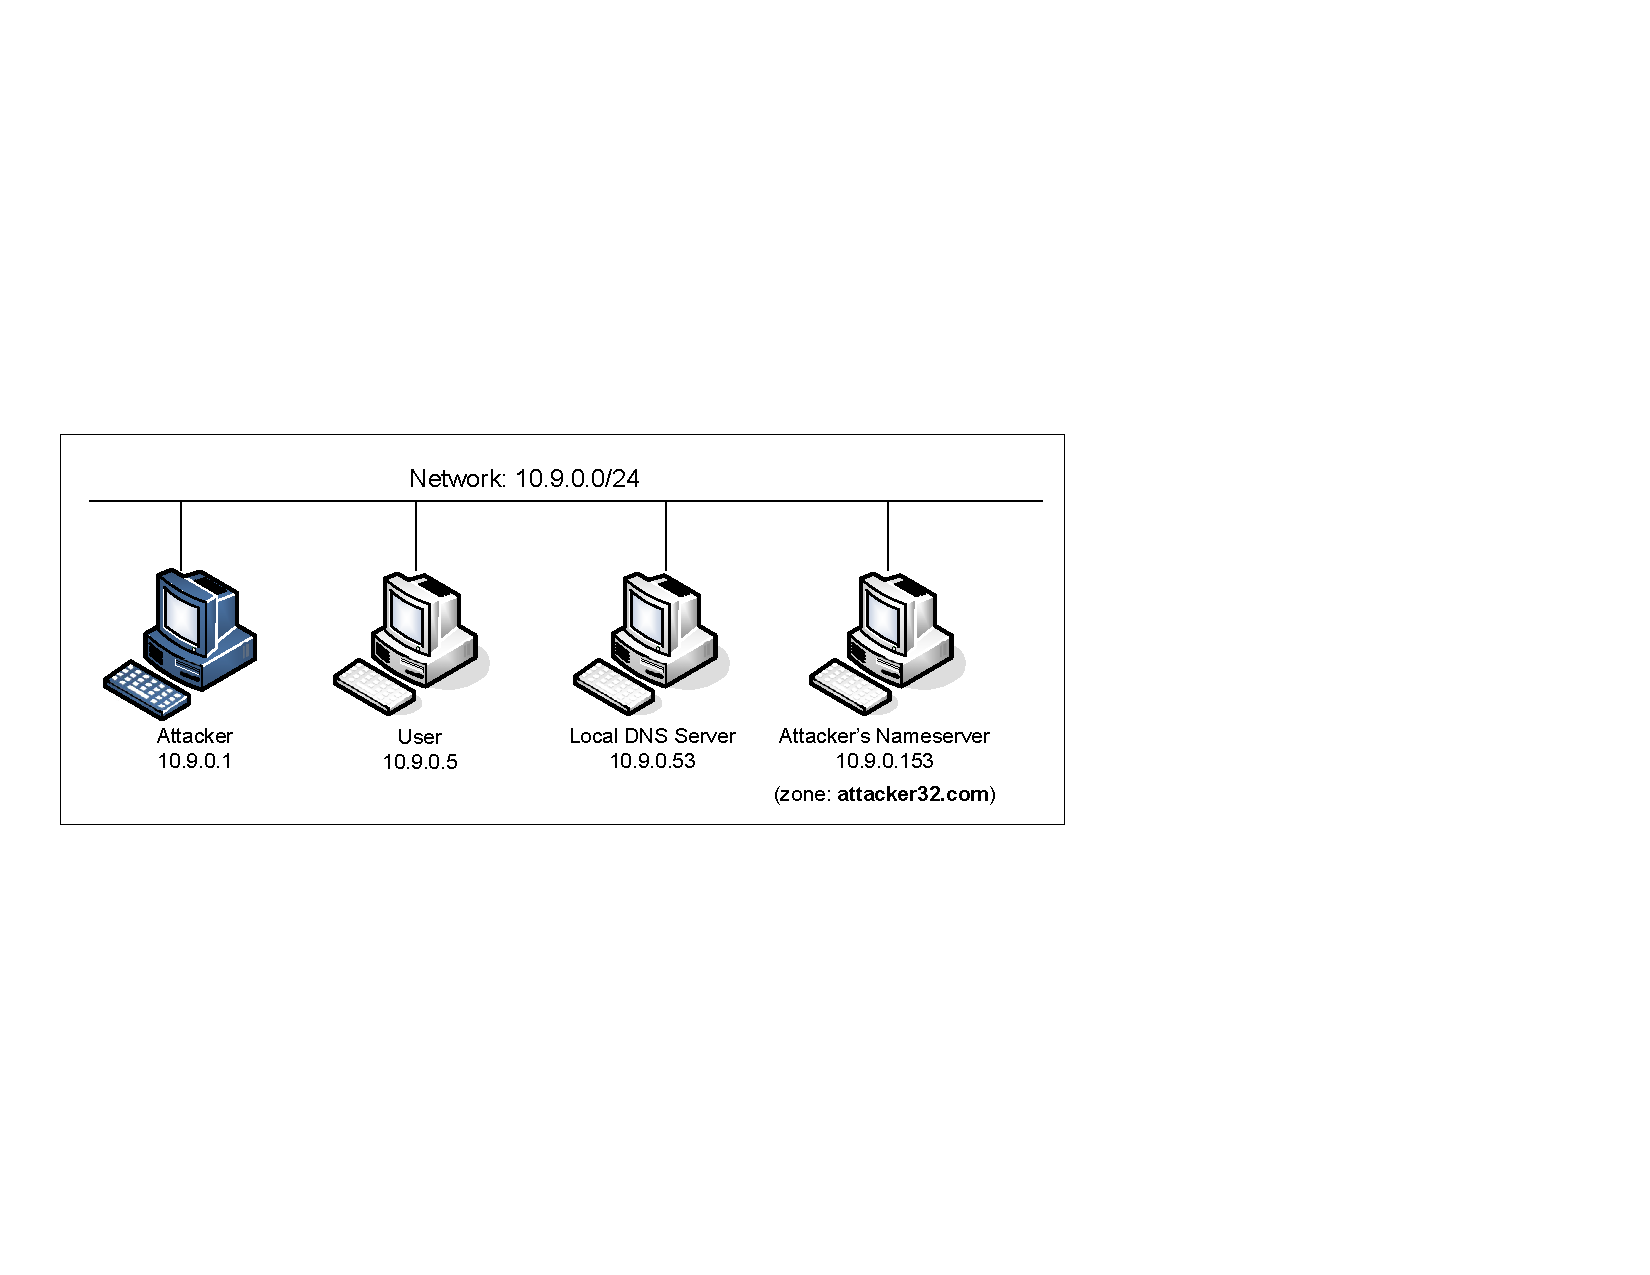
\includegraphics[width=0.85\textwidth]{\commonfolder/Figs/DNS.pdf}
\caption{Environment setup for the experiment}
\label{dns:fig:environment}
\end{figure}


The main target for DNS cache poisoning attacks is
local DNS server.  Obviously, it
is illegal to attack a real server, so we need to set up our own DNS
server to  conduct the attack experiments. The lab
environment needs four separate machines:
one for the victim, one for the DNS server, and two for the attacker.
The lab environment setup is illustrated in Figure~\ref{dns:fig:environment}.



%\begin{lstlisting}[backgroundcolor=]
% +------------+   +------------+  +------------+  +---------------+
% | Attack VM  |   |  Container |  |  Container |  |  Container    |
% |            |   |   (user)   |  |  Local DNS |  |attacker32.com |
% |            |   |            |  |   Server   |  |  nameserver   |
% |  10.9.0.1  |   |  10.9.0.5  |  |  10.9.0.53 |  |  10.9.0.153   |
% +-----+------+   +------+-----+  +------+-----+  +------+--------+
%       |                 |               |               |
%       |                 |               |               |
%-------+-----------------+---------------+---------------+-------
%           Network  10.9.0.0/24
%
%\end{lstlisting}

We put all these machines on the same LAN only for the sake of simplicity. 
Students are not allowed to exploit this fact in their attacks; 
they should treat the attacker machine as a remote machine, 
i.e., the attacker cannot sniff packets on the LAN. 
This is different from the local DNS attack. 


% -------------------------------------------
% SUBSECTION
% -------------------------------------------
\subsection{Container Setup and Commands}


%%%%%%%%%%%%%%%%%%%%%%%%%%%%%%%%%%%%%%%%%%%%
Please download the
\texttt{Labsetup.zip} file to your VM from the lab's website,
unzip it, enter the \texttt{Labsetup} folder, and 
use the \texttt{docker-compose.yml} file to 
set up the lab environment. Detailed explanation
of the content in this file and all the involved 
\texttt{Dockerfile} can be found from the 
user manual, which is linked to the website of this lab.
If this is the first time you set up a SEED lab environment
using containers, it is very important that you read 
the user manual. 

In the following, we list some of the commonly
used commands related to Docker and Compose. 
Since we are going to use 
these commands very frequently, we have created aliases for them
in the \texttt{.bashrc} file (in our provided SEEDUbuntu 20.04 VM).


\begin{lstlisting}
$ docker-compose build  # Build the container image
$ docker-compose up     # Start the container
$ docker-compose down   # Shut down the container

// Aliases for the Compose commands above
$ dcbuild       # Alias for: docker-compose build
$ dcup          # Alias for: docker-compose up
$ dcdown        # Alias for: docker-compose down
\end{lstlisting}


All the containers will be running in the background. To run
commands on a container, we often need to get a shell on
that container. We first need to use the \texttt{"docker ps"}  
command to find out the ID of the container, and then
use \texttt{"docker exec"} to start a shell on that 
container. We have created aliases for them in
the \texttt{.bashrc} file.

\begin{lstlisting}
$ dockps        # Alias for: docker ps --format "{{.ID}}  {{.Names}}" 
$ docksh <id>   # Alias for: docker exec -it <id> /bin/bash

# The following example shows how to get a shell inside hostC
$ dockps
b1004832e275  hostA-10.9.0.5
0af4ea7a3e2e  hostB-10.9.0.6
9652715c8e0a  hostC-10.9.0.7

$ docksh 96
root@9652715c8e0a:/#  

# Note: If a docker command requires a container ID, you do not need to 
#       type the entire ID string. Typing the first few characters will 
#       be sufficient, as long as they are unique among all the containers. 
\end{lstlisting}


If you encounter problems when setting up the lab environment, 
please read the ``Common Problems'' section of the manual
for potential solutions.


%%%%%%%%%%%%%%%%%%%%%%%%%%%%%%%%%%%%%%%%%%%%



% -------------------------------------------
% SUBSECTION
% -------------------------------------------
\subsection{About the Attacker Container}

In this lab, we can either use the VM or the attacker container
as the attacker machine. If you look at the Docker Compose file, you will
see that the attacker container is configured differently from the other
containers.


\begin{itemize}
\item \textit{Shared folder.} When we use the attacker container
to launch attacks, we need to put the attacking code inside
the attacker container.
%%%%%%%%%%%%%%%%%%%%%%%%%%%%%%%%%%%%%%%%%%%%%%%
Code editing is more convenient inside the VM than in a container, 
because we can use our favorite editor to write code. 
In order for the VM and a container to share files, 
we have created a shared folder between VM and the container
using the Docker \texttt{volumes}.
If you look at the Docker Compose file, you will find out that
we have added the following entry to some of the containers.
It indicates mounting the \texttt{./volumes} folder on the host
machine (i.e., the VM) to the \texttt{/volumes} folder inside the container.
We will write our code in the \texttt{./volumes} folder (on the VM), so they
can be used inside the containers.

\begin{lstlisting}
volumes:
       - ./volumes:/volumes
\end{lstlisting}


%%%%%%%%%%%%%%%%%%%%%%%%%%%%%%%%%%%%%%%%%%%%%%%


\item \textit{Host mode.}
%%%%%%%%%%%%%%%%%%%%%%%%%%%%%%%%%%%%%%%%%%%%%%%
In this lab, the attacker needs to be able to sniff packets,
but running sniffer programs inside a container has problems, because
a container is effectively attached to a virtual switch, 
so it can only see its own traffic, and it is never going to see 
the packets among other containers. To solve this problem,
we use the \texttt{host} mode for the attacker container. This
allows the attacker container to see all the traffics. The following
entry used on the attacker container:

\begin{lstlisting}
network_mode: host
\end{lstlisting}

When a container is in the \texttt{host} mode,  it sees
all the host's network interfaces, and it even has the same
IP addresses as the host. Basically, it is put in the
same network namespace as the host VM. However, the container
is still a separate machine, because its other namespaces are
still different from the host.


%%%%%%%%%%%%%%%%%%%%%%%%%%%%%%%%%%%%%%%%%%%%%%%
\end{itemize}





% -------------------------------------------
% SUBSECTION
% -------------------------------------------
%%%%%%%%%%%%%%%%%%%%%%%%%%%%%%%%%%%%%%%%%%%%
%%%%%%%%%%%%%%%%%%%%%%%%%%%%%%%%%%%%%%%%%%%%%%%%%%%%%%%%%%%%%%%%%%%%%%
%%  Copyright by Wenliang Du.                                       %%
%%  This work is licensed under the Creative Commons                %%
%%  Attribution-NonCommercial-ShareAlike 4.0 International License. %%
%%  To view a copy of this license, visit                           %%
%%  http://creativecommons.org/licenses/by-nc-sa/4.0/.              %%
%%%%%%%%%%%%%%%%%%%%%%%%%%%%%%%%%%%%%%%%%%%%%%%%%%%%%%%%%%%%%%%%%%%%%%


% -------------------------------------------
% SUBSECTION
% ------------------------------------------- 
\subsection{Summary of the DNS Configuration} 

All the containers are already configured for this lab. 
We provide a summary here, so students are aware of 
these configurations. Detailed explanation
of the configuration can be found from the manual (Section \manualdns).



\paragraph{Local DNS Server.} 
We run the BIND 9 DNS server program on the local DNS server. 
BIND 9 gets its configuration from a file called \path{/etc/bind/named.conf}. This file
is the primary configuration file, and it usually contains several \texttt{"include"}
entries, i.e., the actual configurations are stored in those included files. One of the
included files is called \path{/etc/bind/named.conf.options}. 
This is where the actual configuration is set. 


\begin{itemize}
\item \textit{Simplification.}
DNS servers now randomize
the source port number in their DNS queries; this makes the attacks much more
difficult. Unfortunately, many DNS servers still use predictable source
port number.  For the sake of simplicity in this lab, we fix the
source port number to  {\tt 33333} in the 
configuration file. 

\item \textit{Turning off DNSSEC.} 
DNSSEC is introduced to protect against spoofing attacks on DNS servers.
To show how attacks work
without this protection mechanism, we have turned off the protection 
in the configuration file. 


\item \textit{DNS cache.}
During the attack, we need to inspect the DNS cache on the local DNS server.
The following two commands are related to DNS cache.
The first command dumps the content of the cache to the file 
\path{/var/cache/bind/dump.db}, 
and the second command clears the cache.

\begin{lstlisting}
# rndc dumpdb -cache    // Dump the cache to the specified file
# rndc flush            // Flush the DNS cache
\end{lstlisting}

\item \textit{Forwarding the \texttt{attacker32.com} zone.}
A forward zone is added to the local DNS server,
so if anybody queries the \texttt{attacker32.com} domain, 
the query will be forwarded to this domain's nameserver, which
is hosted in the attacker container. The zone entry
is put inside the \texttt{named.conf} file. 

\begin{lstlisting}
zone "attacker32.com" {
    type forward;
    forwarders { 
        10.9.0.153; 
    };
};
\end{lstlisting}
\end{itemize}



\paragraph{User machine.}
The user container {\tt 10.9.0.5} is already 
configured to use {\tt 10.9.0.53} as its local DNS server.
This is achieved by changing
the resolver configuration file~(\texttt{/etc/resolv.conf}) of the user machine,
so the server \texttt{10.9.0.53} is added as the first \texttt{nameserver} entry in the file, i.e.,
this server will be used as the primary DNS server.


\paragraph{Attacker's Nameserver.}
On the attacker's nameserver, we host two zones. One is 
the attacker's legitimate zone \texttt{attacker32.com}, and the other 
is the fake \texttt{example.com} zone. The zones are 
configured in \path{/etc/bind/named.conf}:

\begin{lstlisting}
zone "attacker32.com" {
        type master;
        file "/etc/bind/attacker32.com.zone";
};

zone "example.com" {
        type master;
        file "/etc/bind/example.com.zone";
};
\end{lstlisting}


%%%%%%%%%%%%%%%%%%%%%%%%%%%%%%%%%%%%%%%%%%%%%%%%%%%%%%%%%%%%%%%%%%%%%%
%%  Copyright by Wenliang Du.                                       %%
%%  This work is licensed under the Creative Commons                %%
%%  Attribution-NonCommercial-ShareAlike 4.0 International License. %%
%%  To view a copy of this license, visit                           %%
%%  http://creativecommons.org/licenses/by-nc-sa/4.0/.              %%
%%%%%%%%%%%%%%%%%%%%%%%%%%%%%%%%%%%%%%%%%%%%%%%%%%%%%%%%%%%%%%%%%%%%%%


% -------------------------------------------
% SUBSECTION
% ------------------------------------------- 
\subsection{Testing the DNS Setup}

From the User container, we will run a series of commands to ensure 
that our lab setup is correct. In your lab report, please document
your testing results. 


\paragraph{Get the IP address of \texttt{ns.attacker32.com}.}
When we run the following \texttt{dig} command, 
the local DNS server will forward the request to the Attacker nameserver 
due to the \texttt{forward} zone entry added to the local DNS server's
configuration file. Therefore, the answer should come from
the \texttt{attacker32.com.zone} file that we set up on the Attacker nameserver.
If this is not what you get, your setup has an issue. Please describe your
observation in your lab report. 

\begin{lstlisting}
$ dig ns.attacker32.com
\end{lstlisting}



\paragraph{Get the IP address of \texttt{www.example.com}.} 
Two nameservers are now hosting the \texttt{example.com} 
domain, one is the domain's official nameserver, and the other 
is the Attacker container. We will query these two nameservers and see what 
response we will get. 
Please run the following two commands (from the User machine), 
and describe your observation. 


\begin{lstlisting}
// Send the query to our local DNS server, which will send the query
// to example.com's official nameserver. 
$ dig www.example.com

// Send the query directly to ns.attacker32.com 
$ dig @ns.attacker32.com www.example.com
\end{lstlisting}
 


Obviously, nobody is going to ask \texttt{ns.attacker32.com} for 
the IP address of \texttt{www.example.com}; they will always ask
the \texttt{example.com} domain's official nameserver for 
answers. The objective of the DNS cache poisoning attack
is to get the victims to ask 
\texttt{ns.attacker32.com} for the IP address of 
\texttt{www.example.com}. Namely, if our attack is successful, 
if we just run the first \texttt{dig} command, the one
without the \texttt{@} option, we should get the 
fake result from the attacker, instead of getting 
the authentic one from the domain's legitimate nameserver.



%%%%%%%%%%%%%%%%%%%%%%%%%%%%%%%%%%%%%%%%%%%%



% *******************************************
% SECTION
% ******************************************* 
\section{The Attack Tasks}


The main objective of DNS attacks is to redirect the user
to another machine $B$ when the user tries to get to machine $A$ using
$A$'s host name. For example, assuming {\tt www.example.com} is an online banking 
site.  When the user tries to access this site using the
correct URL {\tt www.example.com}, if the adversaries can redirect the user 
to a malicious web site that looks very much like 
{\tt www.example.com}, the user might be fooled and give away 
his/her credentials to the attacker. 


In this task, we use the domain name {\tt www.example.com}
as our attacking target. It should be noted that the {\tt example.com} 
domain name is reserved for use in documentation, not for 
any real company. The authentic IP address of {\tt www.example.com} is 
{\tt 93.184.216.34}, and its nameserver is managed by
the Internet Corporation for Assigned Names and Numbers (ICANN).
When the user runs the {\tt dig} command 
on this name or types the name in the browser, 
the user's machine sends a DNS query to its local DNS 
server, which will eventually ask for the IP address 
from {\tt example.com}'s nameserver. 


The goal of the attack is to launch the DNS cache poisoning attack
on the local DNS server, such that 
when the user runs the {\tt dig} command to find out {\tt
www.example.com}'s IP address, the local DNS server will end
up going to the attacker's nameserver {\tt ns.attacker32.com} 
to get the IP address, so the IP address returned can be 
any number that is decided by the attacker. As results, the 
user will be led to the attacker's web site,
instead of to the authentic {\tt www.example.com}.




\begin{figure}[htb]
\centering
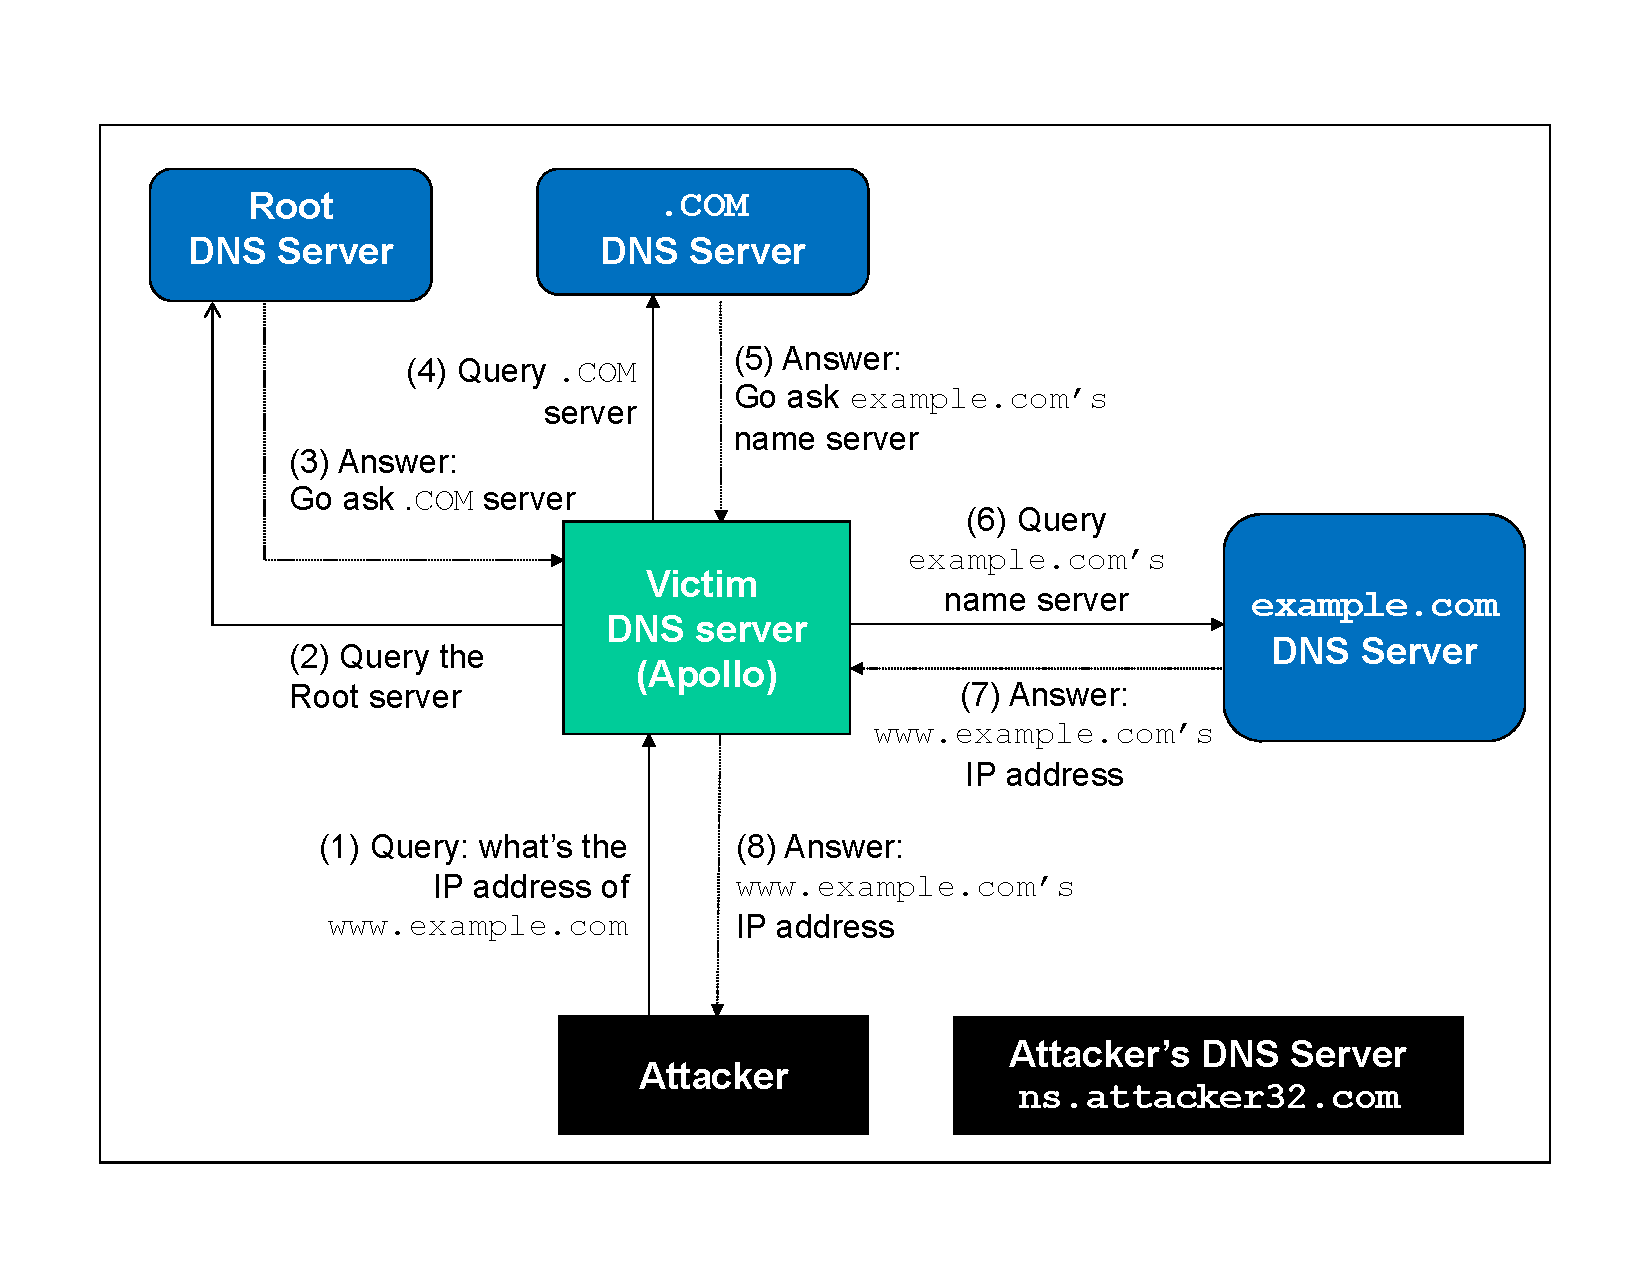
\includegraphics[width=0.9\textwidth]{\dnsFigs/DNS_Remote_new1.pdf}
\caption{The complete DNS query process} 
\label{fig:flow_diagram1}
\end{figure}


\begin{figure}[htb]
\centering
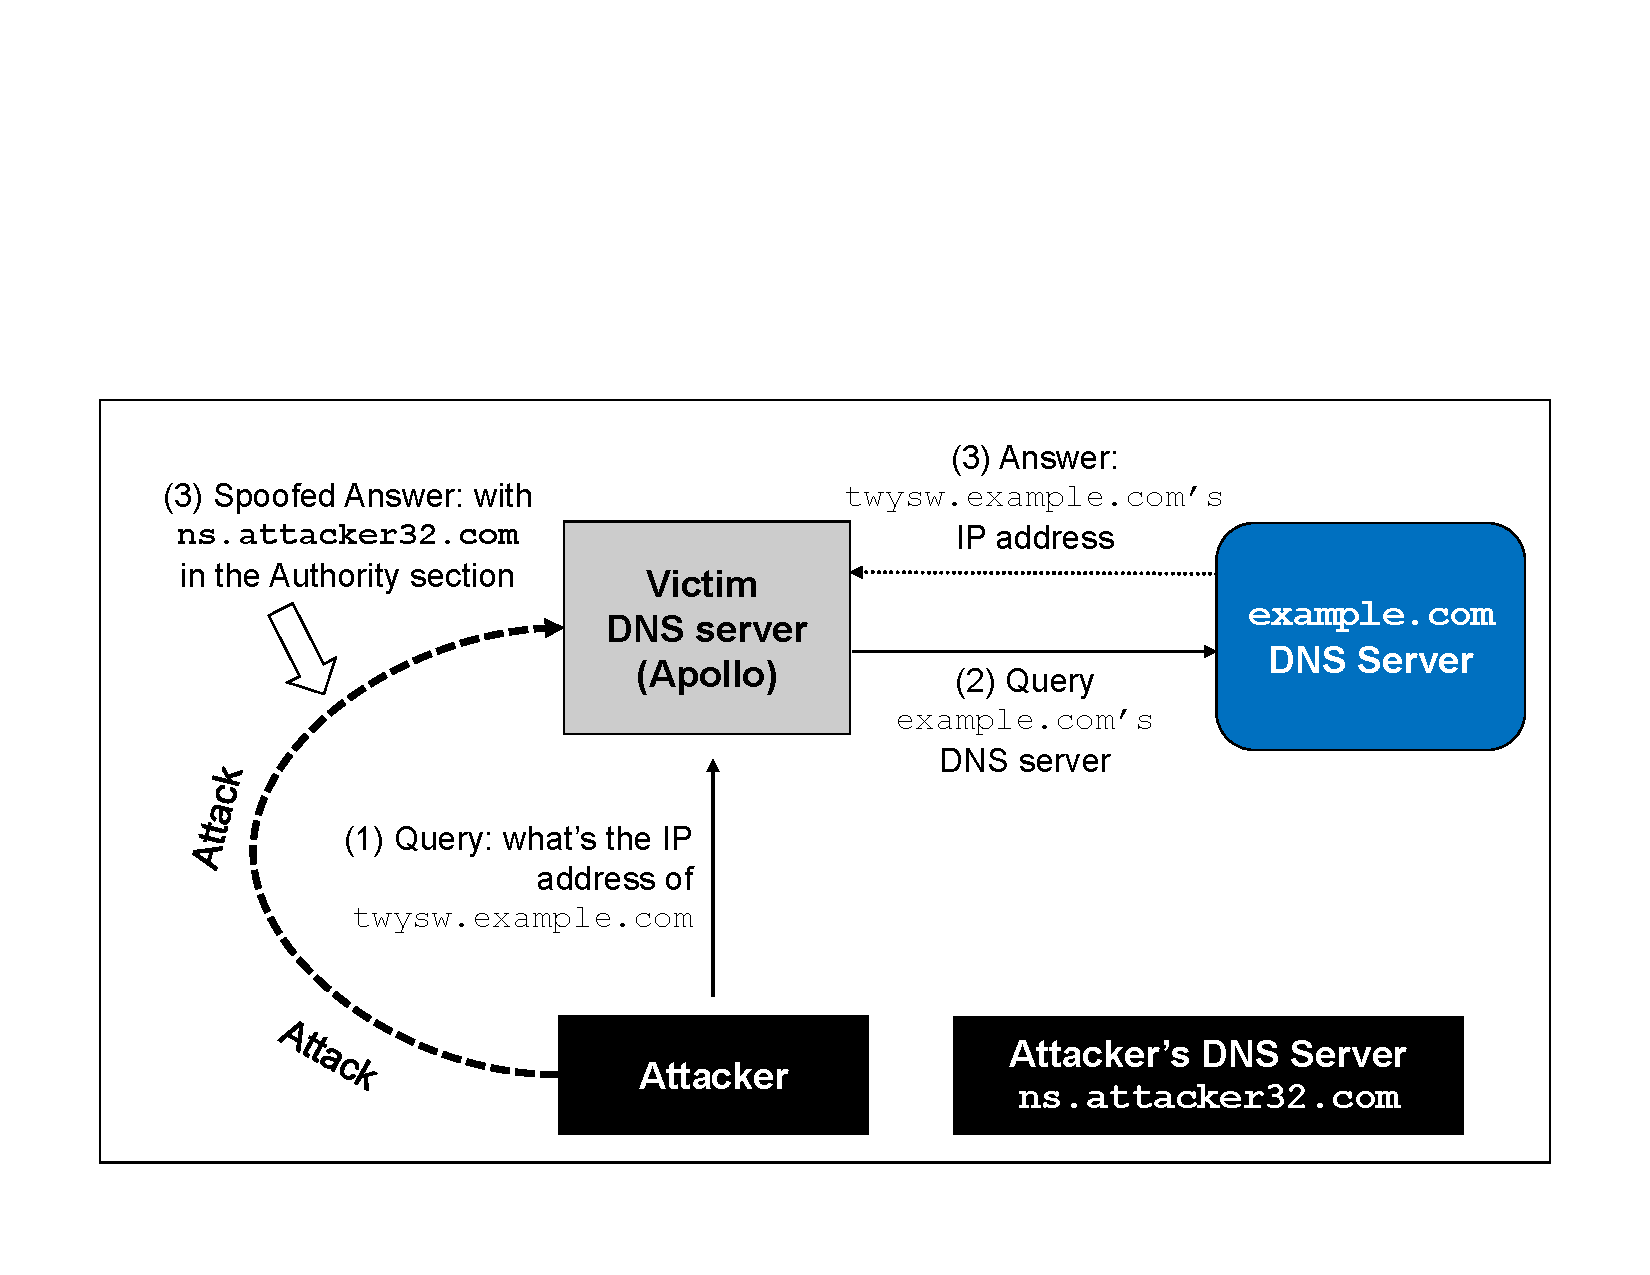
\includegraphics[width=0.9\textwidth]{\dnsFigs/DNS_Remote_new2.pdf}
\caption{The Kaminsky Attack}
\label{fig:flow_diagram2}
\end{figure}



% -------------------------------------------
% SUBSECTION
% ------------------------------------------- 
\subsection{How Kaminsky attack works}

In this task, the attacker sends a DNS query request to the victim
DNS server ({\tt Apollo}), triggering a DNS query from {\tt Apollo}. The
query may go through one of the root DNS servers, the {\tt .COM} DNS server, and 
the final result will come back from {\tt example.com}'s DNS server. This 
is illustrated in Figure~\ref{fig:flow_diagram1}. In case that 
{\tt example.com}'s nameserver information is already cached by 
{\tt Apollo}, the query will not go through the root or the 
{\tt .COM} server; this is illustrated in Figure~\ref{fig:flow_diagram2}.
In this lab, the situation depicted in  Figure~\ref{fig:flow_diagram2} is 
more common, so we will use this figure as the basis to describe 
the attack mechanism.

While {\tt Apollo} waits for the DNS reply from {\tt example.com}'s name
server, the attacker can send forged replies to {\tt Apollo}, pretending 
that the replies are from {\tt example.com}'s nameserver. If the forged 
replies arrive first, it will be accepted by {\tt Apollo}. The attack will
be successful.


If you have done our local DNS attack lab, you should realize that 
those attacks assume that the attacker and the DNS server are on
the same LAN, i.e., the attacker can observe the DNS query message. 
When the attacker and the DNS server are not on the same LAN,
the cache poisoning attack becomes more difficult.
The difficulty is mainly caused by the fact that the transaction ID
in the DNS response packet must match with that 
in the query packet. Because the transaction ID in the query is 
usually randomly generated, without seeing the query packet,
it is not easy for the attacker to know the correct ID.


Obviously, the attacker can guess the transaction ID. Since the
size of the ID is only 16 bits, if the attacker can forge $K$ 
responses within the attack window (i.e. before the legitimate
response arrives), the probability of success is $K$ over $2^{16}$.
Sending out hundreds of forged responses is not impractical, so
it will not take too many tries before the attacker can succeed. 


However, the above hypothetical attack has overlooked the cache effect.
In reality, if the attacker is not fortunate enough to make a correct guess before
the real response packet arrives, correct information will be cached 
by the DNS server for a while. This caching effect makes it impossible
for the attacker to forge another response regarding the same 
name, because the DNS server will not send out another DNS query for 
this name before the cache times out.
To forge another response on the same name, the attacker has to 
wait for another DNS query on this name, which means he/she has to
wait for the cache to time out. The waiting period can be hours or days.


\paragraph{The Kaminsky Attack.} 
Dan Kaminsky came up with an elegant technique to defeat the caching
effect~\cite{dns:Kaminsky}.
With the Kaminsky attack, attackers will be able to continuously attack
a DNS server on a domain name, without the need for waiting, so
attacks can succeed within a very short period of time.
Details of the attacks are described in~\cite{dns:Kaminsky,seedbook}. 
In this task, we will try this attack method. The following steps with reference to 
Figure~\ref{fig:flow_diagram2} outlines the attack. 

\begin{enumerate}
\item The attacker queries the DNS Server {\tt Apollo} for a non-existing name in 
{\tt example.com}, such as {\tt twysw.example.com},
where {\tt twysw} is a random name. 

\item Since the mapping is unavailable in {\tt Apollo}'s DNS cache, 
{\tt Apollo} sends a DNS query to the nameserver of
the {\tt example.com} domain.

\item While {\tt Apollo} waits for the reply, 
the attacker floods {\tt Apollo} with a stream of spoofed DNS response,
each trying a different transaction ID, hoping one is correct.
In the response, not only does the attacker provide an IP resolution
for {\tt twysw.example.com}, the attacker 
also provides an ``Authoritative Nameservers'' record, indicating 
{\tt ns.attacker32.com} as the nameserver for the {\tt example.com} domain.
If the spoofed response beats the actual responses and
the transaction ID matches with that in the query, 
{\tt Apollo} will accept and cache the spoofed answer, and
and thus {\tt Apollo}'s DNS cache is poisoned.  

\item Even if the spoofed DNS response fails (e.g.
the transaction ID does not match or it comes too late),
it does not matter, because the next time, the attacker will query
a different name, so {\tt Apollo} has to send out another query, 
giving the attack another chance to do the spoofing attack. 
This effectively defeats the caching effect.


\item If the attack succeeds, in {\tt Apollo}'s DNS cache, the
nameserver for {\tt example.com} will be replaced by the attacker's
nameserver {\tt ns.attacker32.com}.
To demonstrate the success of this attack, students need to show that such a record 
is in {\tt Apollo}'s DNS cache. 

\end{enumerate}


\paragraph{Task overview.} Implementing the Kaminsky attack is quite challenging, 
so we break it down into several sub-tasks. 
In Task 2, we construct the DNS request for a random hostname 
in the \texttt{example.com} domain. In Task 3, we construct a spoofed 
DNS reply from \texttt{example.com}'s nameserver.
In Task 4, we put everything together to launch the 
Kaminsky attack. Finally in Task 5, we verify the impact of the attack. 


% -------------------------------------------
% SUBSECTION
% ------------------------------------------- 
\subsection{Task 2: Construct DNS request} 

This task focuses on sending out DNS requests. 
In order to complete the attack, attackers need to trigger the target 
DNS server to send out DNS queries, so they have a chance 
to spoof DNS replies. Since attackers need to try many times before they 
can succeed, it is better to automate the process using a program. 

Students need to write a program to send out DNS queries to the target DNS 
server (i.e., the local DNS server in our setup). 
Students' job is to write this program
and demonstrate (using Wireshark) that their queries can
trigger the target DNS server to send out corresponding DNS queries.
The performance requirement for this task is not high, so
students can use C or Python (using Scapy) to write this code. 
A Python code snippet is provided in the following (the 
\texttt{+++}'s are placeholders; students need to replace them
with actual values): 

\begin{lstlisting}
Qdsec  = DNSQR(qname='www.example.com')
dns    = DNS(id=0xAAAA, qr=0, qdcount=1, ancount=0, nscount=0,
             arcount=0, qd=Qdsec)

ip  = IP(dst='+++', src='+++')
udp = UDP(dport=+++, sport=+++, chksum=0)
request = ip/udp/dns
\end{lstlisting}
 


% -------------------------------------------
% SUBSECTION
% ------------------------------------------- 
\subsection{Task 3: Spoof DNS Replies.}   

In this task, we need to spoof DNS replies in the Kaminsky attack. 
Since our target is \texttt{example.com}, we need to spoof
the replies from this domain's nameserver. Students first need to 
find out the IP addresses of \texttt{example.com}'s legitimate 
nameservers (it should be noted that there are multiple 
nameservers for this domain).

Students can use Scapy to implement this task. The following 
code snippet constructs a DNS response packet that includes 
a question section, an answer section, and an NS section. 
In the sample code, we use \texttt{+++} as placeholders; 
students need to replace them with the correct values 
that are needed in the Kaminsky attack. Students need to explain
why they pick those values. 

\begin{lstlisting}
name   = '+++'  
domain = '+++'  
ns     = '+++'

Qdsec  = DNSQR(qname=name)
Anssec = DNSRR(rrname=name,   type='A',  rdata='1.2.3.4', ttl=259200)
NSsec  = DNSRR(rrname=domain, type='NS', rdata=ns, ttl=259200)
dns    = DNS(id=0xAAAA, aa=1, rd=1, qr=1,
             qdcount=1, ancount=1, nscount=1, arcount=0,
             qd=Qdsec, an=Anssec, ns=NSsec)

ip    = IP(dst='+++', src='+++')
udp   = UDP(dport=+++, sport=+++, chksum=0)
reply = ip/udp/dns
\end{lstlisting}
 

Since this reply by itself will not be able to lead to a successful 
attack, to demonstrate this task, students need to 
use Wireshark to capture the spoofed DNS replies, and 
show that the spoofed packets are valid. 


% -------------------------------------------
% SUBSECTION
% ------------------------------------------- 
\subsection{Task 4: Launch the Kaminsky Attack}   

Now we can put everything together to conduct the Kaminsky attack. 
In the attack, we need to send out many spoofed DNS replies, hoping 
one of them hits the correct transaction number and arrives sooner
than the legitimate replies. Therefore, speed is essential: the more packets 
we can send out, the higher the success rate is. If we use 
Scapy to send the spoofed DNS replies like what we did in the 
previous task, the success rate is too low. Students can use 
C, but constructing DNS packets in C is non-trivial. 
We introduce a hybrid approach using both Scapy and C (see the SEED
book for details). 


With the hybrid approach, we first use Scapy to generate 
a DNS packet template, which is stored in a file. 
We then load this template into a C program, and make 
small changes to some of the fields, and then send 
out the packet. 
We have included a skeleton C code
in \path{Labsetup/Files/attack.c}. 
Students can make changes
in the marked areas. Detailed explanation
of the code is given in the 
guideline section.


\paragraph{Check the DNS cache.}
To check whether the attack is successful or not, we need to 
check the {\tt dump.db} file to see whether our spoofed DNS
response has been successfully accepted by the DNS server. 
The following commands dump the DNS cache, and search whether
the cache contains the word \texttt{attacker} (in our 
attack, we used \texttt{attacker32.com} as the attacker's 
domain; if students use a different domain name, they should 
search for a different word).  

\begin{lstlisting}
# rndc dumpdb -cache && grep attacker /var/cache/bind/dump.db
\end{lstlisting}
 

% -------------------------------------------
% SUBSECTION
% ------------------------------------------- 
\subsection{Task 5: Result Verification}

If the attack is successful, in the local DNS server's DNS cache, 
the {\tt NS} record for \texttt{example.com} will become 
\texttt{ns.attacker32.com}.
When this server receives a DNS query for any hostname
inside the \texttt{example.com} domain,  it will
send a query to \texttt{ns.attacker32.com}, instead of 
sending to the domain's legitimate nameserver. 


To verify whether your attack is successful or not, 
go to the User machine, run the following two
\texttt{dig} commands. In the responses, the IP addresses for 
\texttt{www.example.com} should be the same for both 
commands, and it should be whatever you have included
in the zone file on the Attacker nameserver. 

\begin{lstlisting}
// Ask the local DNS server to do the query
$ dig www.example.com

// Directly query the attacker32 nameserver
$ dig @ns.attacker32.com www.example.com
\end{lstlisting}
 
Please include your observation (screenshots) in the lab 
report, and explain why you think your attack is successful. 
In particular, when you run the first \texttt{dig} commands,
use Wireshark to capture the network traffic, and 
point out what packets are triggered by this
\texttt{dig} command. Use the packet trace to 
prove that your attack is successful. Note that DNS results
may be cached on the local DNS server after the first
\texttt{dig} command is run. This could influence the
results if you run the first \texttt{dig} command before using
Wireshark. You can clear the cache using \texttt{"sudo rndc flush"} 
on the local DNS server, but that will 
require you to redo the attack.



% *******************************************
% SECTION
% ******************************************* 
\section{Guidelines} 

To implement the Kaminsky attack, we can use Scapy to do the packet spoofing. Unfortunately,
the speed of Python is too slow; the number of packets generated per second is too low to
make the attack successful. It is better to use a C program. This could
be quite challenging to many students, because constructing DNS packets using C is not very
easy. I have developed a hybrid method, and have experimented with it in my own class. Using
this approach, students' time spent on coding can be significantly reduced, so they can spend
more time focusing on the actual attack.


The idea is to leverage the strength of both Scapy and C: Scapy is much more convenient in
creating DNS packets than C, but C is much faster. Therefore we simply
use Scapy to create the spoofed DNS packet, and save it to a file.
We then load the packet into a C program. Even though we need to send a 
lot of different DNS packets
during the Kaminsky attack, these packets are mostly the same, except for a few fields. 
Therefore, we can
use the packet generated from Scapy as the basis, find the offsets where
changes need to be made (e.g., the transaction ID field),
and directly make changes. This will be much easier than
creating the entire DNS packets in C.
After the changes are made, we can use the raw socket to send out the packets.
Details of such a hybrid method are provided in
the Packet Sniffing and Spoofing chapter 
of the SEED book~\cite{seedbook}.
The following Scapy program creates a simple DNS reply packet, 
and saves it into a file.


\begin{lstlisting}[caption={\texttt{generate\_dns\_reply.py}}]
#!/usr/bin/env python3
from scapy.all import *

# Construct the DNS header and payload
name   = 'twysw.example.com'
Qdsec  = DNSQR(qname=name)
Anssec = DNSRR(rrname=name, type='A', rdata='1.1.2.2', ttl=259200)
dns    = DNS(id=0xAAAA, aa=1, rd=0, qr=1, 
             qdcount=1, ancount=1, nscount=0, arcount=0, 
             qd=Qdsec, an=Anssec)

# Construct the IP, UDP headers, and the entire packet
ip  = IP(dst='10.0.2.7', src='1.2.3.4', chksum=0)
udp = UDP(dport=33333, sport=53, chksum=0)
pkt = ip/udp/dns

# Save the packet to a file
with open('ip.bin', 'wb') as f:
  f.write(bytes(pkt))
\end{lstlisting}

In a C program, we load the packet from the file \texttt{ip.bin}, and use
it as our packet template, based on which we create many similar packets,
and flood the target local DNS servers with these spoofed replies. For each
reply, we change three places: the transaction ID and the name
\texttt{twysw} occurred in two places (the question section and the answer
section).  The transaction ID is at a fixed place (offset  \texttt{28} from
the beginning of our IP packet), but the offset for the name \texttt{twysw}
depends on the length of the domain name. We can use a binary editor
program, such as \texttt{bless}, to view the binary file \texttt{ip.bin}
and find the two offsets of \texttt{twysw}. In our packet, they are at
offsets \texttt{41} and \texttt{64}.


The following code snippet shows how we make change to these fields. We change
the name in our reply to \texttt{bbbbb.example.com}, and then send out a
spoofed DNS replies, with transaction ID being \texttt{1000}.
In the code, the variable \texttt{ip} points to the beginning of the IP packet.  

\begin{lstlisting}
  // Modify the name in the question field (offset=41)
  memcpy(ip+41, "bbbbb" , 5);

  // Modify the name in the answer field (offset=64)
  memcpy(ip+64, "bbbbb" , 5);

  // Modify the transaction ID field (offset=28)
  unsigned short id = 1000;
  unsigned short id_net_order = htons(id);
  memcpy(ip+28, &id_net_order, 2);
\end{lstlisting}



\paragraph{Generate random names.} In the Kaminsky attack, we need to 
generate random hostnames. There are many ways to do so. The following 
code snippet shows how to generate a random name consisting of 
5 characters. 

\begin{lstlisting}
char a[26]="abcdefghijklmnopqrstuvwxyz";

// Generate a random name of length 5
char name[6];
name[5] = 0;
for (int k=0; k<5; k++)  
   name[k] = a[rand() % 26];
\end{lstlisting}
 



% *******************************************
% SECTION
% ******************************************* 
\section{Submission}

%%%%%%%%%%%%%%%%%%%%%%%%%%%%%%%%%%%%%%%%

You need to submit a detailed lab report, with screenshots,
to describe what you have done and what you have observed.
You also need to provide explanation
to the observations that are interesting or surprising.
Please also list the important code snippets followed by
explanation. Simply attaching code without any explanation will not
receive credits.

%%%%%%%%%%%%%%%%%%%%%%%%%%%%%%%%%%%%%%%%



%%%%%%%%%%%%%%%%%%%%%%%%%%%%%%%%%%%%%%%%%%
\thispagestyle{empty}
\bibliographystyle{plain}
\def\baselinestretch{1}
\bibliography{BibDNS}
%%%%%%%%%%%%%%%%%%%%%%%%%%%%%%%%%%%%%%%%%%



\end{document}
%%%%%%%%%%%%%%%%%%%%%%%%%%%%%%%%%%%%%%%%%%%
%%%%%%%%%%%%%%%%%%%%%%%%%%%%%%%%%%%%%%%%%%%
%%%%%%%%%%%%%%%%%%%%%%%%%%%%%%%%%%%%%%%%%%%
%%%%%%%%%%%%%%%%%%%%%%%%%%%%%%%%%%%%%%%%%%%
%%%%%%%%%%%%%%%%%%%%%%%%%%%%%%%%%%%%%%%%%%%
%%%%%%%%%%%%%%%%%%%%%%%%%%%%%%%%%%%%%%%%%%%
%%%%%%%%%%%%%%%%%%%%%%%%%%%%%%%%%%%%%%%%%%%



